\documentclass[a4paper,12pt]{article}

% Packages
\usepackage{graphicx}   % Required for inserting images
\usepackage{hyperref}   % Required for clickable links and ToC
\usepackage{geometry}   % Better page margins
\usepackage{booktabs}   % For professional looking tables
\usepackage{listings}   % For code snippets
\usepackage{xcolor}     % For code coloring
\usepackage{float}      % improved interface for floating objects
\usepackage{tikz}       % Diagrams
\usetikzlibrary{positioning,arrows.meta,shapes.geometric}

% Setup for code snippets
\lstset{
    basicstyle=\ttfamily\small,
    backgroundcolor=\color{gray!10},
    frame=single,
    breaklines=true,
    keywordstyle=\color{blue},
    commentstyle=\color{green!50!black},
    stringstyle=\color{red}
}

% setup hyperlink colors
\hypersetup{
    colorlinks=true,
    linkcolor=black,
    filecolor=magenta,      
    urlcolor=blue,
    pdftitle={ESP32-CAM and Hand Gesture LED Control Documentation},
}

% Project Metadata
\title{\textbf{ESP32-CAM and Hand Gesture LED Control}}
\author{Stefan-Daniel Horvath}
\date{February 2026}

\begin{document}

\maketitle

% The Table of Contents
\tableofcontents
\newpage

\section{Project Description}
The project combines an \textbf{ESP32-CAM} camera board with Python vision scripts and an \textbf{ESP32 LED strip} controller. The ESP32-CAM serves an MJPEG video stream over WiFi. A PC runs Python scripts that consume this stream for object counting, face detection, or hand gesture recognition. 
The hand gesture script controls a separate ESP32-driven addressable LED strip over HTTP: open palm turns lights on, OK gesture turns them off, thumbs up/down adjust brightness, and index finger (pointer) drives fun mode (moving cluster position and hue) where pinching triggers a tetris like stacking effect.

Optional ways to start the different scripts include \texttt{gesture\_launcher.py} (a small UI to paste camera and LED strip IPs and start the hand gesture script) and \texttt{run.ps1} (PowerShell launcher that creates a virtual environment, installs dependencies, and runs a chosen script).

\subsection{Key Features}
\begin{itemize}
    \item \textbf{MJPEG stream:} ESP32-CAM serves \texttt{/stream} and a minimal HTML viewer at \texttt{/}
    \item \textbf{Shared stream reader:} \texttt{stream\_reader.py} parses MJPEG or polls snapshot URLs for compatibility with ESP32-CAM
    \item \textbf{Object counting:} Blob counting on contrasting background with optional click-to-set background and tunable parameters
    \item \textbf{Face detection:} OpenCV Haar cascade; optional face recognition via \texttt{face\_recognition} and \texttt{known\_faces/}
    \item \textbf{Hand gestures:} MediaPipe Hand Landmarker; open palm = on, OK = off, thumbs = brightness, pointer = fun mode
    \item \textbf{LED strip control:} HTTP API (on/off, fun position/hue, brightness); serial commands for the LED board
    \item \textbf{Launcher:} \texttt{run.ps1} for venv and script selection; \texttt{gesture\_launcher.py} for camera/LED IPs and Start
\end{itemize}

\section{Links}
\begin{itemize}
    \item \textbf{MediaPipe:} \href{https://developers.google.com/mediapipe}{developers.google.com/mediapipe} (Hand Landmarker)
    \item \textbf{OpenCV:} \href{https://opencv.org/}{https://opencv.org/}
    \item \textbf{ESP32-CAM / Arduino:} \href{https://github.com/espressif/arduino-esp32}{https://github.com/espressif/arduino-esp32}
    \item \textbf{Adafruit NeoPixel:} \href{https://github.com/adafruit/Adafruit\_NeoPixel}{github.com/adafruit/Adafruit\_NeoPixel} (WS2812B strips)
\end{itemize}

\section{Hardware}

\subsection{Bill of Materials (BOM)}
Two ESP32-based units are used: the camera server and the LED strip controller.

\begin{center}
\begin{tabular}{@{}lll@{}}
\toprule
\textbf{Component} & \textbf{Model/Type} & \textbf{Quantity} \\ \midrule
ESP32-CAM (camera) & AI Thinker, OV2640   & 1 \\ \midrule
ESP32 (LED controller) & ESP32 dev board     & 1 \\
LED strip            & WS2812B/NeoPixel or simple digital & 1 \\\bottomrule
\end{tabular}
\end{center}

\subsection{ESP32-CAM}
The camera runs \texttt{main.ino}: connects to WiFi, serves MJPEG at \texttt{/stream} and a minimal HTML page at \texttt{/}. Resolution and pins are set in the sketch (e.g.\ \texttt{esp32cam::Resolution::find(1280,720)}, \texttt{pins::AiThinker}). No extra wiring beyond power and antenna; the board exposes the camera and WiFi.

\subsection{ESP32 LED Strip}
The esp32 controller connected to the LED strip runs \texttt{esp32\_led\_strip.ino} in the \texttt{esp32\_led\_strip} folder. Wiring:
\begin{itemize}
    \item \textbf{LED data:} GPIO 4 (\texttt{LED\_PIN}) to strip data input
    \item \textbf{Power:} 5V and GND to strip power (separate supply recommended for long strips but the VCC and GND on the esp32 can be used)
    \item \textbf{Strip type:} \texttt{USE\_WS2812 = 1} for WS2812B/NeoPixel; \texttt{USE\_WS2812 = 0} for simple digital on/off
\end{itemize}
Set \texttt{NUM\_LEDS} to match your strip length. For WS2812, install the Adafruit NeoPixel library in the Arduino Library Manager.

\section{Software Overview}

\subsection{Firmware}
\begin{itemize}
    \item \texttt{main.ino} -- ESP32-CAM: WiFi, camera init, \texttt{/stream} (MJPEG) and \texttt{/} (HTML viewer)
    \item \texttt{esp32\_led\_strip/esp32\_led\_strip.ino} -- ESP32: HTTP server for \texttt{/on}, \texttt{/off}, \texttt{/fun}, \texttt{/brightness/up}, \texttt{/brightness/down}, \texttt{/}; serial commands \texttt{on}, \texttt{off}, \texttt{status}, \texttt{bright+}, \texttt{bright-}
\end{itemize}

\subsection{Python Scripts}
\begin{itemize}
    \item \texttt{stream\_reader.py} -- Shared MJPEG/snapshot reader; yields BGR frames; \texttt{add\_stream\_url\_arg()} for CLI
    \item \texttt{object\_count.py} -- Counts blobs (contours) on contrasting background; optional background from click
    \item \texttt{face\_detect.py} -- Face detection (Haar); optional recognition with \texttt{known\_faces/}
    \item \texttt{hand\_gesture.py} -- MediaPipe hands, gesture classification, LED HTTP commands
    \item \texttt{gesture\_launcher.py} -- Tkinter UI: camera URL, LED URL, mirror/webcam; starts \texttt{hand\_gesture.py}
\end{itemize}

\subsection{Launcher}
\texttt{run.ps1} takes a script name (\texttt{object\_count}, \texttt{face\_detect}, \texttt{hand\_gesture}, \texttt{gesture\_launcher}), ensures a \texttt{.venv} exists (Python 3.9+ for hand\_gesture/gesture\_launcher), runs \texttt{pip install -r requirements.txt}, sets \texttt{PYTHONPATH}, and runs the corresponding \texttt{.py} script with any extra arguments.

\subsection{Libraries to install}
\textbf{Python} (install via \texttt{pip install -r requirements.txt} in the project \texttt{.venv}):
\begin{itemize}
    \item \texttt{opencv-python} (>=4.8.0) -- used by all vision scripts (stream\_reader, object\_count, face\_detect, hand\_gesture)
    \item \texttt{requests} (>=2.28.0) -- HTTP for stream and LED strip
    \item \texttt{mediapipe} (>=0.10.0) -- hand landmarks for \texttt{hand\_gesture.py} (requires Python 3.9+)
    \item \texttt{face\_recognition} (>=1.3.0) -- optional; uncomment in \texttt{requirements.txt} to enable \texttt{face\_detect.py --recognize}
\end{itemize}

\textbf{Arduino / ESP32} (install via Arduino Library Manager or PlatformIO):
\begin{itemize}
    \item \texttt{main.ino}: \texttt{WebServer}, \texttt{WiFi} (ESP32 core), \texttt{esp32cam} (camera and stream). Add \texttt{secrets.h} with \texttt{ssid} and \texttt{password}.
    \item \texttt{esp32\_led\_strip.ino}: \texttt{WebServer}, \texttt{WiFi}; if \texttt{USE\_WS2812 = 1}, install \texttt{Adafruit NeoPixel}. Add \texttt{secrets.h} with WiFi credentials.
\end{itemize}

\section{Environment and Dependencies}

\subsection{Python}
Requires Python 3.9+ for \texttt{hand\_gesture.py} (MediaPipe 0.10+).  It has to be installed on the PC before being able to run anything, and it can be installed on windows machines by typing ``python'' in the terminal, which will open the windows app store. 
\\Then from the project directory:
\begin{lstlisting}[language=bash]
python -m venv .venv
.venv\Scripts\activate   # Windows
pip install -r requirements.txt
\end{lstlisting}
\texttt{requirements.txt} includes \texttt{opencv-python}, \texttt{requests}, \texttt{mediapipe}. Uncomment \texttt{face\_recognition} in \texttt{requirements.txt} to enable \texttt{face\_detect.py --recognize}.

\subsection{Arduino / ESP32}
\begin{itemize}
    \item ESP32 board support (Arduino IDE or PlatformIO)
    \item \texttt{main.ino}: \texttt{WebServer}, \texttt{WiFi}, \texttt{esp32cam} (and \texttt{secrets.h} for \texttt{ssid}/\texttt{password})
    \item \texttt{esp32\_led\_strip.ino}: \texttt{WebServer}, \texttt{WiFi}; for WS2812 add Adafruit NeoPixel
\end{itemize}
Both sketches expect a \texttt{secrets.h} (or equivalent) with \texttt{ssid} and \texttt{password} for WiFi.

\subsection{Configuration}
\begin{itemize}
    \item \textbf{Stream URL:} Set via \texttt{--url} or \texttt{STREAM\_URL} (default \texttt{http://192.168.1.100/stream}). \texttt{stream\_reader} appends \texttt{/stream} if missing.
    \item \textbf{LED strip:} \texttt{--led-url} for \texttt{hand\_gesture.py}; e.g.\ \texttt{http://192.168.1.101}
    \item \textbf{Gesture launcher:} Saves/loads camera and LED URLs and options in \texttt{.gesture\_launcher\_config.txt}
\end{itemize}

\section{Architecture and Diagrams}

\subsection{System Architecture}
Figure \ref{fig:system} shows the high-level flow: ESP32-CAM streams MJPEG to the PC; Python scripts use \texttt{stream\_reader} to get frames; \texttt{hand\_gesture} sends HTTP requests to the ESP32 LED strip. The launcher and \texttt{run.ps1} are optional entry points.

\begin{figure}[ht]
\centering
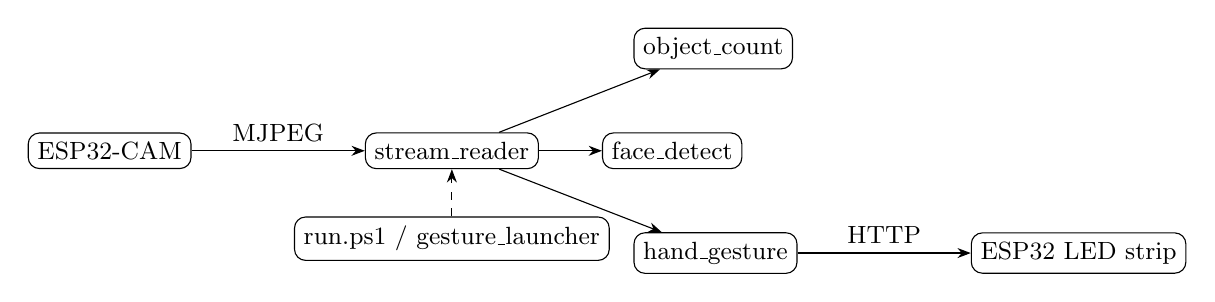
\begin{tikzpicture}[node distance=1.2cm,>=Stealth,every node/.style={font=\small}]
  \node[draw,rectangle,rounded corners] (cam) {ESP32-CAM};
  \node[draw,rectangle,rounded corners,right=2.2cm of cam] (reader) {stream\_reader};
  \node[draw,rectangle,rounded corners,above right=0.8cm and 1.2cm of reader] (obj) {object\_count};
  \node[draw,rectangle,rounded corners,right=0.8cm of reader] (face) {face\_detect};
  \node[draw,rectangle,rounded corners,below right=0.8cm and 1.2cm of reader] (hand) {hand\_gesture};
  \node[draw,rectangle,rounded corners,right=2.2cm of hand] (led) {ESP32 LED strip};
  \node[draw,rectangle,rounded corners,below=0.6cm of reader] (run) {run.ps1 / gesture\_launcher};

  \draw[->] (cam) -- node[above] {MJPEG} (reader);
  \draw[->] (reader) -- (obj);
  \draw[->] (reader) -- (face);
  \draw[->] (reader) -- (hand);
  \draw[->] (hand) -- node[above] {HTTP} (led);
  \draw[->,dashed] (run) -- (reader);
\end{tikzpicture}
\caption{System architecture: camera stream to Python scripts; hand gesture script controls LED strip.}
\label{fig:system}
\end{figure}

\subsection{Stream to Script Data Flow}
Figure \ref{fig:stream} shows how frames reach the scripts: HTTP GET to \texttt{/stream} (or a snapshot URL) is parsed by \texttt{stream\_reader} (MJPEG boundary parse or single-JPEG poll) into BGR frames, which are consumed by object\_count, face\_detect, or hand\_gesture.

\begin{figure}[ht]
\centering
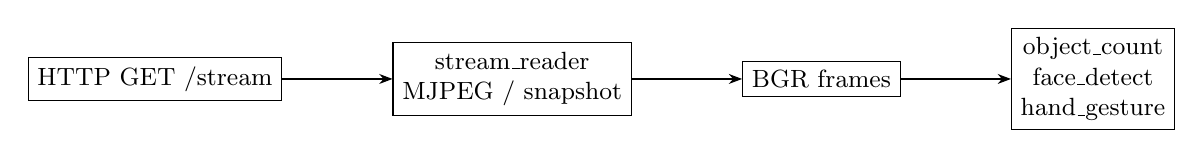
\begin{tikzpicture}[node distance=1.4cm,>=Stealth,every node/.style={font=\small,align=center}]
  \node[draw,rectangle] (http) {HTTP GET /stream};
  \node[draw,rectangle,right=of http] (parse) {stream\_reader\\MJPEG / snapshot};
  \node[draw,rectangle,right=of parse] (frames) {BGR frames};
  \node[draw,rectangle,right=of frames] (scripts) {object\_count\\face\_detect\\hand\_gesture};

  \draw[->] (http) -- (parse);
  \draw[->] (parse) -- (frames);
  \draw[->] (frames) -- (scripts);
\end{tikzpicture}
\caption{Data flow from stream URL to vision scripts.}
\label{fig:stream}
\end{figure}

\subsection{Hand Gesture Pipeline}
Figure \ref{fig:gesture} summarizes the hand gesture path: frames go to MediaPipe Hand Landmarker, finger states are computed, a gesture is classified, and the corresponding action is sent to the LED strip via HTTP (on/off, brightness, fun).

\begin{figure}[ht]
\centering
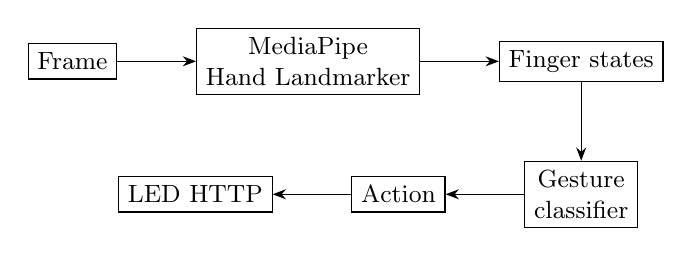
\begin{tikzpicture}[node distance=1cm,>=Stealth,every node/.style={font=\small,align=center,draw,rectangle}]
  % Row 1: left to right
  \node (frame) {Frame};
  \node (mp) [right=of frame] {MediaPipe\\Hand Landmarker};
  \node (fingers) [right=of mp] {Finger states};
  % Row 2: right to left (so flow continues naturally)
  \node (gesture) [below=of fingers] {Gesture\\classifier};
  \node (action) [left=of gesture] {Action};
  \node (led) [left=of action] {LED HTTP};

  \draw[->] (frame) -- (mp);
  \draw[->] (mp) -- (fingers);
  \draw[->] (fingers) -- (gesture);
  \draw[->] (gesture) -- (action);
  \draw[->] (action) -- (led);
\end{tikzpicture}
\caption{Hand gesture pipeline from frame to LED commands.}
\label{fig:gesture}
\end{figure}

\subsection{run.ps1 Flow}
Figure \ref{fig:runps1} outlines the launcher: script name and arguments trigger venv creation (if missing), Python 3.9+ check for hand\_gesture/gesture\_launcher, dependency install, \texttt{PYTHONPATH} set, and script execution.

\begin{figure}[ht]
\centering
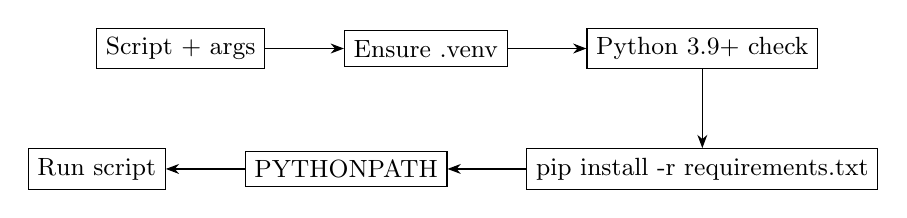
\begin{tikzpicture}[node distance=1cm,>=Stealth,every node/.style={font=\small,draw,rectangle}]
  % Row 1: left to right
  \node (in) {Script + args};
  \node (venv) [right=of in] {Ensure .venv};
  \node (py) [right=of venv] {Python 3.9+ check};
  % Row 2: right to left
  \node (pip) [below=of py] {pip install -r requirements.txt};
  \node (path) [left=of pip] {PYTHONPATH};
  \node (run) [left=of path] {Run script};

  \draw[->] (in) -- (venv);
  \draw[->] (venv) -- (py);
  \draw[->] (py) -- (pip);
  \draw[->] (pip) -- (path);
  \draw[->] (path) -- (run);
\end{tikzpicture}
\caption{run.ps1 flow from script selection to execution.}
\label{fig:runps1}
\end{figure}

\section{Algorithms Used in the Project}
This section explains how the vision scripts work ``under the hood,'' so the pipeline is a white box rather than a black box.

\subsection{Object Counting (Blob Counting)}
\textbf{Script:} \texttt{object\_count.py}.

The goal is to separate foreground objects from the background and then count connected regions (blobs) whose area lies in a given range.

\textbf{Pipeline (in order):}
\begin{enumerate}
    \item \textbf{Grayscale:} Convert the frame to a single intensity value per pixel.
    \item \textbf{Gaussian blur} (e.g.\ 5$\times$5): Reduces noise so contours are stable and not fragmented.
    \item \textbf{Threshold:} Produce a binary image (foreground vs background).
        \begin{itemize}
            \item \textbf{Otsu's method} (default): Chooses a threshold that best separates two intensity peaks; works well when objects and background have different brightness.
            \item \textbf{Fixed threshold} (e.g.\ 127) or \textbf{click-to-set background}: A pixel is foreground if it differs from a chosen background gray by more than a tolerance.
        \end{itemize}
    \item \textbf{Find contours} (OpenCV \texttt{findContours}, \texttt{RETR\_EXTERNAL}, \texttt{CHAIN\_APPROX\_SIMPLE}): Each contour is the boundary of a connected white region.
    \item \textbf{Filter by area:} Keep only contours with area between \texttt{min\_area} and \texttt{max\_area} (tunable) to ignore tiny noise and huge merged regions.
\end{enumerate}
\textbf{In short:} No machine learning; classic image processing (blur, threshold, contours, area filter). Works best with clear contrast between objects and background.

\subsection{Face Detection and Recognition}
\textbf{Script:} \texttt{face\_detect.py}.

\textbf{Face detection (always on):} The script uses a \textbf{Haar cascade classifier} (OpenCV's \texttt{haarcascade\_frontalface\_default.xml}). A cascade of simple ``Haar-like'' features (e.g.\ edges, contrast in rectangular regions) is applied in a sliding window at multiple scales. Early stages quickly reject non-faces, so only face-like regions get a full evaluation. This is fast and works well for frontal faces in good light. Parameters used: \texttt{scaleFactor=1.1}, \texttt{minNeighbors=5}, \texttt{minSize=(30,30)} control how the image is scaled, how many neighbors support a detection, and the smallest face size.

\textbf{Face recognition (optional, \texttt{--recognize}):} One photo per person is placed in \texttt{known\_faces/} (e.g.\ \texttt{alice.jpg}). The library extracts a \textbf{face encoding} (a 128-dimensional vector summarizing the face) for each. At runtime, for each detected face box the script computes its encoding and compares it (e.g.\ by distance in 128-D space) to the known encodings; if within a \textbf{tolerance} (e.g.\ 0.6), the face is labeled with that person's name; otherwise ``Unknown.''

\textbf{How to use it.} The project includes a \texttt{known\_faces/} folder. Add one photo per person; the \textbf{filename without extension} is the label shown when that person is recognized (e.g.\ \texttt{Stefan.jpg} shows ``Stefan''). Use a clear, frontal face per image; good lighting helps. Run with \texttt{--recognize} and optionally \texttt{--known-faces} to point to another folder. Recognition requires the \texttt{face\_recognition} package (uncomment it in \texttt{requirements.txt} and run \texttt{pip install -r requirements.txt}). Identity is by \emph{name match} to the known encodings only: there is no persistent ``person 1'' / ``person 2'' by order of appearance; without recognition, labels like ``Face 1'' are just the detector's order that frame and can change between frames.

\textbf{Takeaway:} Detection uses a fast cascade of hand-crafted features; recognition uses pre-trained deep face embeddings and nearest-neighbor comparison.

\subsection{Hand Gesture Recognition}
\textbf{Script:} \texttt{hand\_gesture.py}.

\textbf{Step 1 -- Hand landmarks:} \textbf{MediaPipe Hand Landmarker} (a pre-trained model) takes the frame and outputs, per hand, \textbf{21 3D landmarks} (normalized 0--1): wrist, thumb (4 points), and index, middle, ring, pinky (4 points each). No custom training is done in this project.

\textbf{Step 2 -- Finger states:} For each finger, the code decides ``extended'' or ``folded'' using simple geometry. The \textbf{thumb} uses handedness: e.g.\ tip further along the thumb axis than the joint, or tip farther from the wrist than the joint (so it works when the palm faces the camera). For \textbf{index, middle, ring, pinky}, a finger is ``extended'' if the tip is above the PIP joint in image coordinates \textbf{or} the tip is farther from the wrist than the PIP (so pointing sideways still counts as extended).

\textbf{Step 3 -- Gesture classification:} The mapping from finger states to gesture names is \textbf{rule-based}, not a neural network. Examples: \textbf{Pinch} = thumb--index tip distance $<$ about 30\% of ``hand size'' (e.g.\ wrist to middle base), other fingers folded. \textbf{OK} = same pinch distance but middle, ring, pinky extended. \textbf{Fist} = no fingers extended. \textbf{Open hand} = four or more extended. \textbf{Thumb up/down} = only thumb extended; tip vs joint in $y$ distinguishes them. \textbf{Pointer} = index extended, others (except maybe thumb) folded. Similar rules define peace, rock, etc.

\textbf{Step 4 -- Stability:} \textbf{Debouncing:} A gesture is sent to the LED strip only after it has been the same for several consecutive frames (e.g.\ 5), to avoid flicker from brief misdetections.

\textbf{Takeaway:} The ``AI'' is MediaPipe's hand landmark model; the rest is explicit rules on landmarks and finger states, plus debouncing for stable control.

\section{Script Usage}

Run via \texttt{run.ps1} or directly with the project directory on \texttt{PYTHONPATH}: [text in square brackets are comments and should not be included when using the commands in terminal]
\begin{lstlisting}[language=bash]
.\run.ps1 object_count --url http://[ip address]/stream --min-area 500[optional] ...
.\run.ps1 face_detect --url ... --recognize[to make use of images in the known\_faces folder] ...
.\run.ps1 hand_gesture --url ... --led-url http://LED_IP --webcam --mirror[so that the right hand is shown on the right of the screen] ...
.\run.ps1 gesture_launcher [has UI for launching hand_gesture more comfortably] 
\end{lstlisting}
Common flags: \texttt{--url} (stream URL), \texttt{--led-url} (LED strip base URL), \texttt{--webcam} (use local webcam instead of ESP32-CAM), \texttt{--mirror} (mirror display). For object counting, click on the image to set background. For hand gestures, press \texttt{q} to quit and \texttt{m} to toggle mirror.

\section{LED Strip HTTP API}

The ESP32 LED strip controller (\texttt{esp32\_led\_strip.ino}) exposes:

\begin{center}
\begin{tabular}{@{}ll@{}}
\toprule
\textbf{Endpoint} & \textbf{Description} \\ \midrule
GET \texttt{/on}  & Lights on (solid or last fun state) \\
GET \texttt{/off} & Lights off \\
GET \texttt{/fun?p=P\&h=H} & One moving cluster: position \texttt{P} (0--100), hue \texttt{H} (0--360) \\
GET \texttt{/fun?p=P\&h=H\&p2=P2\&h2=H2} & Two clusters (e.g.\ two hands) \\
GET \texttt{/brightness/up}   & Increase brightness \\
GET \texttt{/brightness/down} & Decrease brightness (min enforced) \\
GET \texttt{/} & Status: \texttt{on} or \texttt{off} (plain text) \\ \bottomrule
\end{tabular}
\end{center}

Serial (115200): \texttt{on}, \texttt{off}, \texttt{status} (or \texttt{?}), \texttt{bright+}, \texttt{bright-}.

\section{Gesture Mapping}

Hand gestures that control the LED strip (only these are sent to the strip):

\begin{center}
\begin{tabular}{@{}ll@{}}
\toprule
\textbf{Gesture} & \textbf{Action} \\ \midrule
OPEN\_HAND  & ON \\
OK          & OFF \\
THUMB\_UP   & BRIGHT+ \\
THUMB\_DOWN & BRIGHT- \\
POINTER     & Fun mode: 1 or 2 moving clusters by hand count (index position and hue) \\
PINCH       & Explosion from hand position (1 or 2 hands) \\
\bottomrule
\end{tabular}
\end{center}

\section{File and Module Overview}

\begin{itemize}
    \item \texttt{main.ino} -- ESP32-CAM MJPEG stream server
    \item \texttt{esp32\_led\_strip/esp32\_led\_strip.ino} -- ESP32 LED strip HTTP and serial control
    \item \texttt{stream\_reader.py} -- MJPEG/snapshot frame reader and \texttt{--url} CLI helper
    \item \texttt{object\_count.py} -- Object (blob) counting from stream
    \item \texttt{face\_detect.py} -- Face detection and optional recognition
    \item \texttt{hand\_gesture.py} -- Hand gesture detection and LED control
    \item \texttt{gesture\_launcher.py} -- UI to configure camera/LED URLs and start hand gesture
    \item \texttt{run.ps1} -- PowerShell launcher: venv, dependencies, script selection
    \item \texttt{requirements.txt} -- Python dependencies (opencv-python, requests, mediapipe; optional face\_recognition)
    \item \texttt{secrets.h} -- WiFi credentials for both ESP32 sketches (not in repo; add locally)
\end{itemize}

\end{document}